\documentclass[../main.tex]{subfiles}

\begin{document}

A Fortran program was developed to implement the discrete solution to the transport equation. The source code is included as an attachment to this report. The code uses $\opmat{A} \vec{b} = \opmat{F} \vec{b}$ to converge to the solution. And initial guess value for b is assumed (we use $\vec{f}=1$ for all discrete points but any values could be used but convergence time will vary). Our b vector is then multiplied by the inverse (obtained using LU decomposition) of our A matrix describe in the Methodology section above. We then repeated the matrix multiplication with the newly obtained flux until the ch   ange upon iteration in the eigenvalues and eigenvectors is lower than some minimum error specified.

The program allowed an analysis of a one-dimensional core filled with a multiplying medium. The flux distribution was solved for by iteratively seeking out eigenvalues of the material matrix. 

In addition to finding the flux profile of the slab, the program also finds at what width the material with a specific $\Sigma_f$ and $\Sigma_a$ is critical. It achieves this by nesting the loop described above into an additional loop which tests if $k = 1 \pm error margin$  and slightly changes the width accordingly until $k$ converges to that value. 

Our numerical calculation of the given parameters gave a critical width of \SI{154.79}{\centi\meter}. This was checked against a calculated value of width using the criticality condition $B_g^2 = B_m^2$:

\begin{align*}
    B_g^2 &= B_m^2 \\
    \left( \frac{\pi}{\tilde{a}} \right) &= \frac{\nu \Sigma_f - \Sigma_a}{D} \\
    \tilde{a} &= \pi \sqrt{ \frac{D}{\nu \Sigma_f - \Sigma_a} } \numberthis \label{eq:buckling} \\
    \tilde{a} &= \SI{154.65}{\centi\meter}
\end{align*}

Substituting the values used to perform our numerical calculations, we arrive at a width of $w = \SI{154.65}{\centi\meter}$, a very close match. A plot of $k_{eff}$ vs. slab width can be seen in figure \ref{fig:k_eff_vs_width}.

\begin{figure}
    \centering
    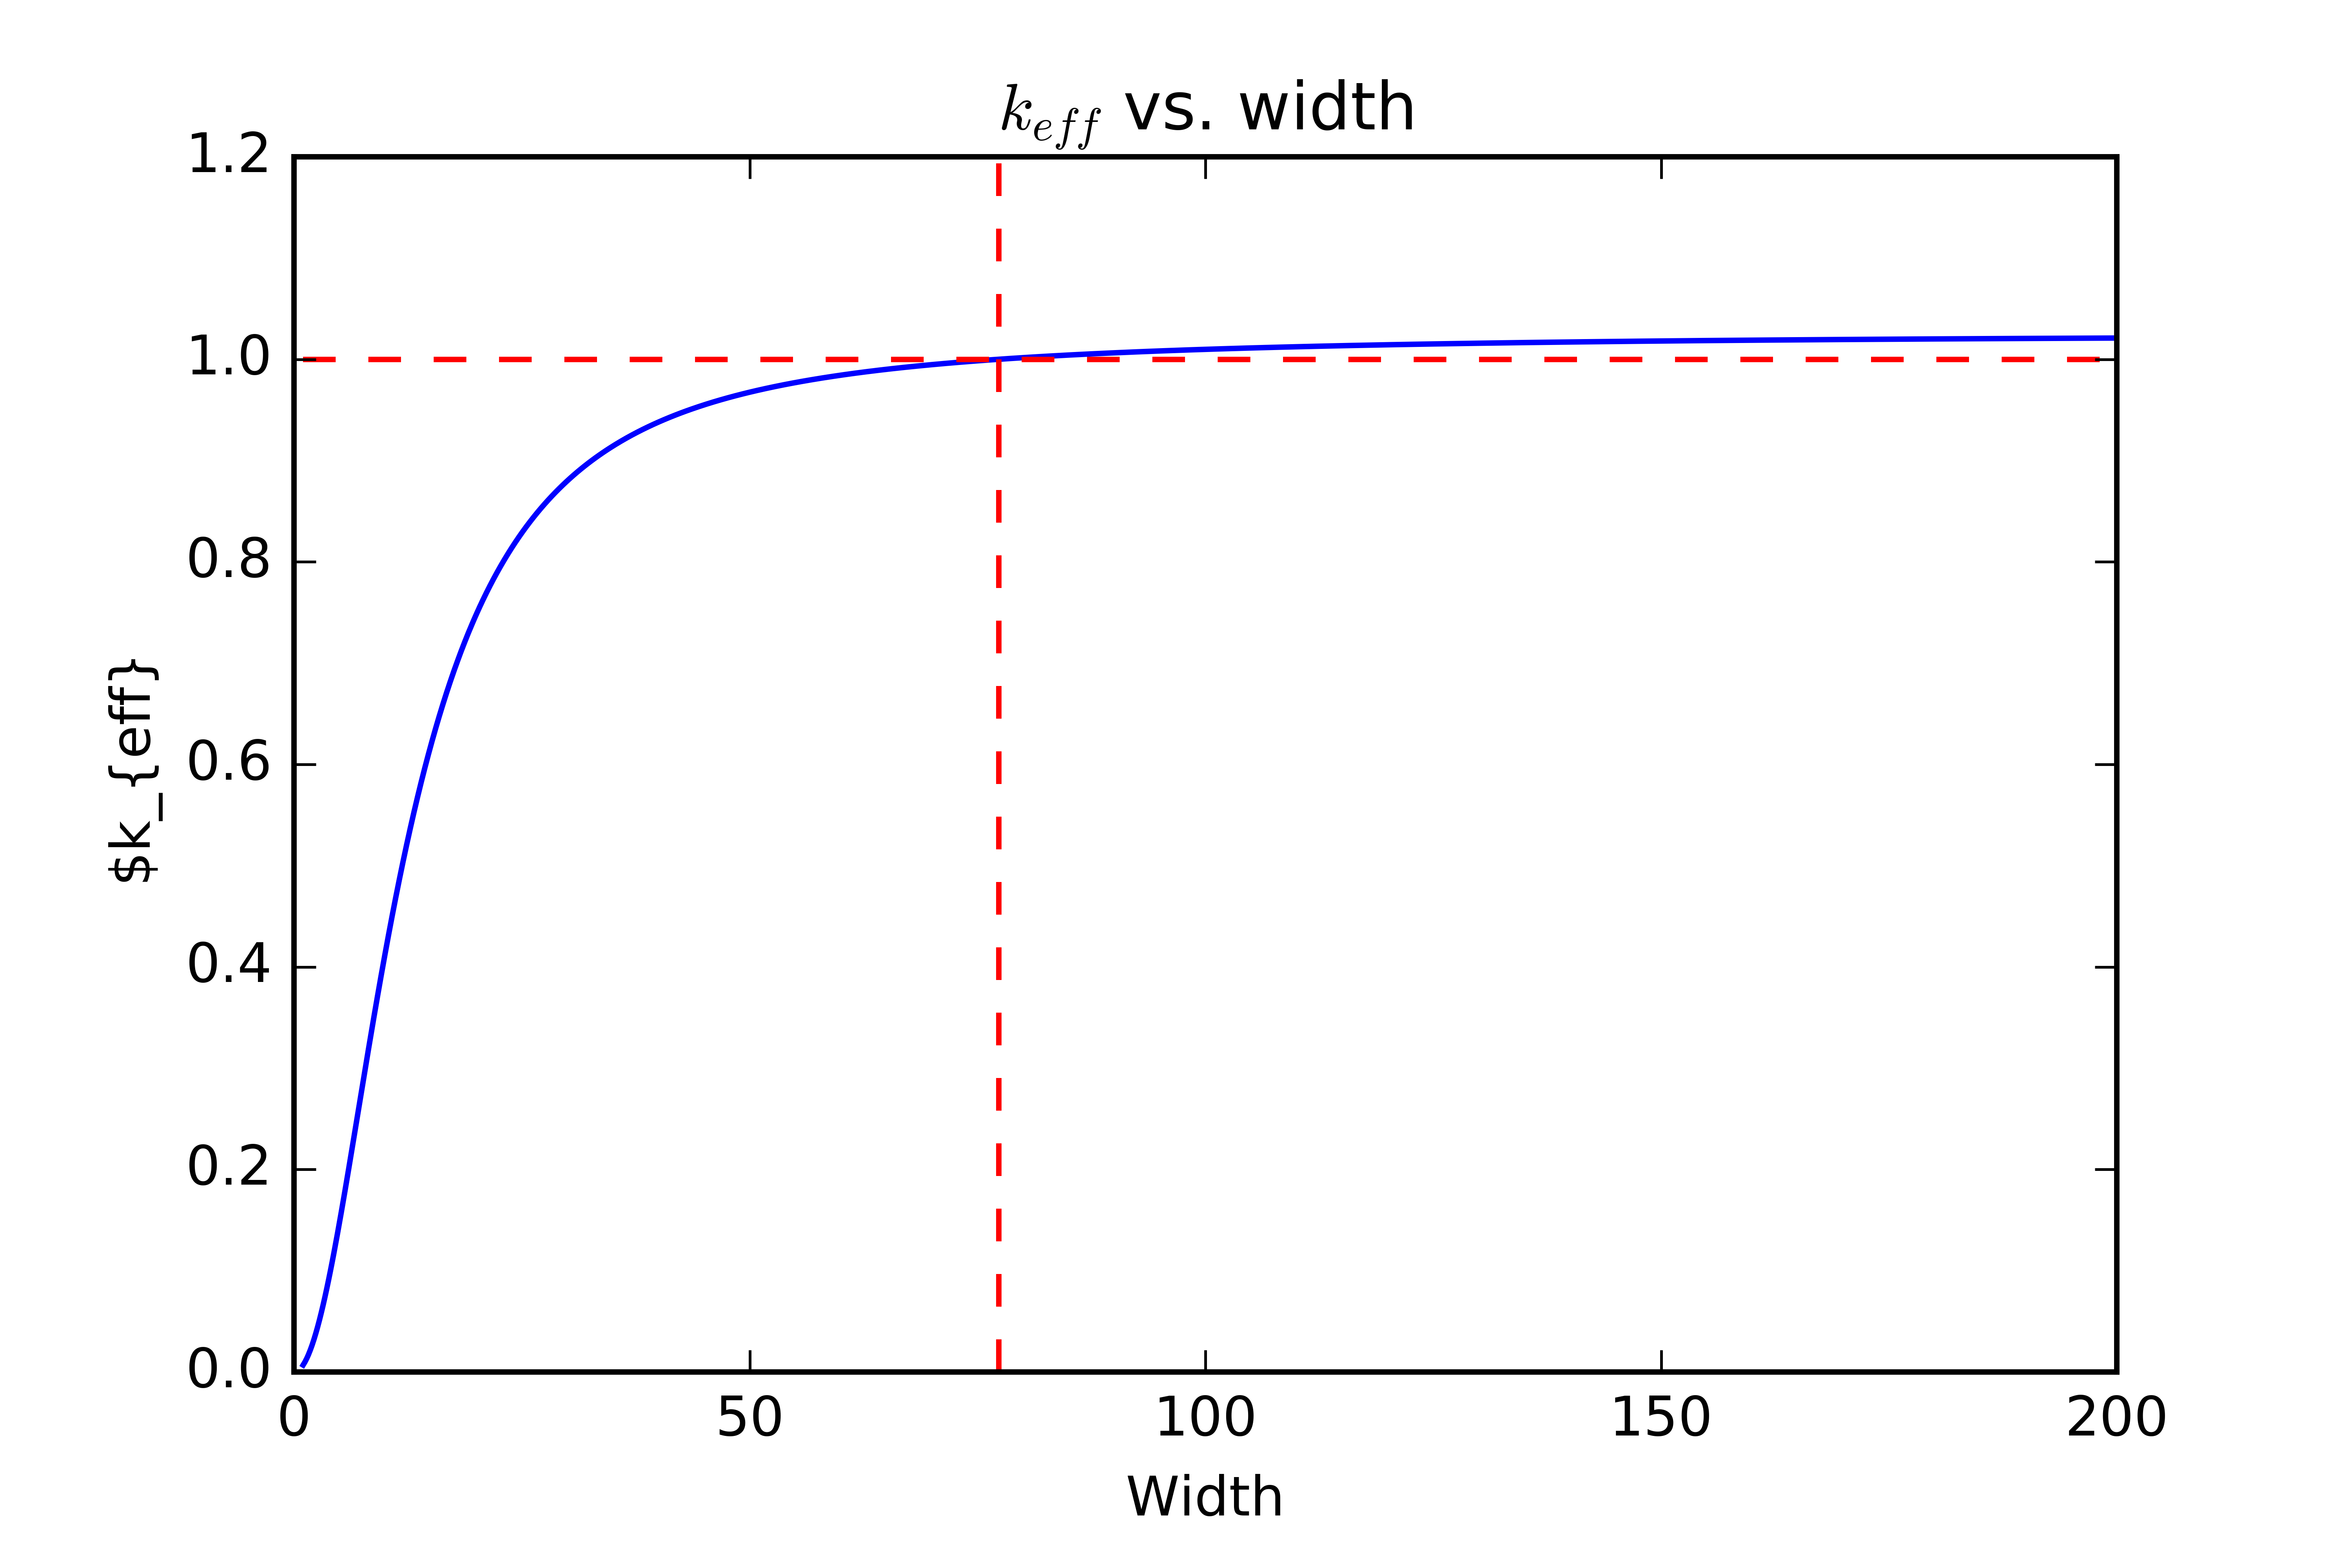
\includegraphics[width=0.75\textwidth]{k_eff_vs_width}
    \caption{$k_eff$ vs. Width}
    \label{fig:k_eff_vs_width}
\end{figure}

As with the previous project, it was worth noting how the values converged as the number of nodes was increased. As such, the program was run with different parameters to determine the convergence. The results of this can be seen in figure \ref{fig:flux_vs_nodes}. From this, it is clear that this method converges by or before $N=500$ nodes, since this appears very similar to $N=10^3$ nodes (allowing for normalization of the flux).

\begin{figure}
\centering
\includegraphics[width=7in]{flux_vs_nodes}
\caption{Normalized Flux vs. Width as a function of the number of nodes}
\label{fig:flux_vs_nodes}
\end{figure}

\end{document}
